\chapter{Grundlagen}\label{basics}
\section{Fazialisparese und House-Brackmann Skala}\label{facialpalsy}
\paragraph{Fazialisparese} (eng. Facial nerve Paralysis) ist eine Funktionsstörung der Hirnnerven und der mimischen Gesichtsmuskulatur. Durch diese Nervenbahnstörung kann eine partielle oder auch vollständige Beeinträchtigung der Muskeln im Gesicht resultieren. Dabei werden vor allem der Lidschluss, Stirnbewegungen (runzeln und Augenbraun heben), Mundwinkel und Lippenschluss als offensichtliche Merkmale negativ beeinflusst. Darüber hinaus können ebenfalls Geschmack, Hörsinn, Speichel und Tränenfluss beeinträchtigt sein. \cite{facialpalsy_1}\cite{facialpalsy_2}.

Die Ursachen für eine mögliche Entwicklung einer Fazialisparese sind dabei genau so fassetttenreich wie deren Ausprägung:
\begin{itemize}
  \setlength\itemsep{-0.5em}
\item Infektionen (z.B. Borrelien)
\item Entzündungen
\item Traumatische oder geburtstraumatische
Schädigung
\item Tumore
\item Angeborener Defekt
\item Idiopathisch (Bell-Parese)
\item Verletzung von Nerven
\end{itemize}

Es gibt verschiedenste Skalen, die eine Einordung für den Schwereverlauf einer vorhandenen Fazialisparese, realisieren. Die bekanntesten Skalen sind dabei Sunnybrook und die House-Brackmann Skala. Im Rahmen der Bachelorarbeit wird allein die House-Brackmann Skala zur Anwendung kommen. Diese ist im Vergleich zu anderen Skalen einfacher im Umgang im zusammenhang mit der Abstufung und Festellung der einzelnen Grade und der späteren Datenausgabe an den behandelnden Arzt*in oder direkt an die Patient*innen. Auch ist diese Skala, aus medizinischer Sicht, ein Standard zur Bewertung der Schwereverlaufes der Fazialisparese \cite{Mothes2019}.




\paragraph{House-Brackmann Skala} ist eine Skala, welche für die Ermittlung des Schweregrades der Fazialisparese Anwendung findet. Diese Skalierungsmethode wurde von John W. House und Derald E. Brackmann 1983 entwickelt. Das System beinhaltet eine 6-Punkte Skala von römisch I Normalzustand bis VI vollständig ausgeprägte Parese (siehe Tabelle \ref{cap:housebrackmann}). Die Einstufung erfolgt, indem der/die Patient*in aufgefordert wird, bestimmte Bewegungen auszuführen. Diese werden durch eine*n Facharzt*in klinisch beobachtet. Daraus resultiert eine subjektive Beurteilung der Schwere der vorliegenden Parese \cite{housebrackmann}.

Ein Vorteil dieser Skala besteht durch die einfache Handhabung, sowie darin, dass alleinig anhand einzelner Figuren und Bewegungsabläufe die Beschreibung der Gesichtsfunktion erfolgen kann. Nachteilhaft sind dabei die subjektive Bewertung des/dem behandelten Arzt*in, sowie dass die regionalen Funktionsunterschiede zwischen dem Grad III und V unempfindlicher für Veränderungen sind Die Subjektivität der Bewertung erschwert dabei zusätzlich eine Vereinheitlichung und die Vergleichbarkeit von Bewertungen durch verschiedene Ärzt*innen.

\begin{table}[!tb]\vspace{1ex}\centering
  \resizebox{0.85\textwidth}{!}{
  \small
  \begin{tabular*}{15.5cm}{c||c||cccc|}
%\hline
\multirow{2}{*}{\textbf{Grad}} &
  \multirow{2}{*}{\textbf{Beschreibung}} &
  \multicolumn{1}{c|}{\textbf{Statisch}} &
  \multicolumn{3}{c|}{\textbf{Dynamisch}} \\ \cline{3-6}
 &
   &
  \multicolumn{1}{c|}{\textbf{Symmetrie}} &
  \multicolumn{1}{c|}{\textbf{Stirn}} &
  \multicolumn{1}{c|}{\textbf{Lidschluss}} &
  \textbf{Mund} \\ \hline\hline
I &
  Normal &
  \multicolumn{4}{c|}{Normal} \\ \hline
II &
  \begin{tabular}[c]{@{}c@{}}Leichte\\ Funktionsstörung\end{tabular} &
  \multicolumn{1}{c|}{Normal} &
  \multicolumn{1}{c|}{\begin{tabular}[c]{@{}c@{}}moderate\\ bis\\ gute\\ Funktion\end{tabular}} &
  \multicolumn{1}{c|}{\begin{tabular}[c]{@{}c@{}}geschlossen,\\ minimale\\ Anstrengung\end{tabular}} &
  \begin{tabular}[c]{@{}c@{}}leichte\\ Asymmetrie\end{tabular} \\ \hline
III &
  \begin{tabular}[c]{@{}c@{}}Moderate\\ Funktionsstörung\end{tabular} &
  \multicolumn{1}{c|}{Normal} &
  \multicolumn{1}{c|}{\begin{tabular}[c]{@{}c@{}}leicht\\ bis\\ moderate\\ Funktion\end{tabular}} &
  \multicolumn{1}{c|}{\begin{tabular}[c]{@{}c@{}}geschlossen,\\ maximale\\ Anstrengung\end{tabular}} &
  \begin{tabular}[c]{@{}c@{}}leicht Betroffen,\\ maximale\\ Anstrengung\end{tabular} \\ \hline
IV &
  \begin{tabular}[c]{@{}c@{}}Mittelschwere\\ Funktionsstörung\end{tabular} &
  \multicolumn{1}{c|}{Normal} &
  \multicolumn{1}{c|}{keine} &
  \multicolumn{1}{c|}{unvollständig} &
  \begin{tabular}[c]{@{}c@{}}Asymmetrisch,\\ maximale\\ Anstrengung\end{tabular} \\ \hline
V &
  \begin{tabular}[c]{@{}c@{}}Schwere\\ Funktionsstörung\end{tabular} &
  \multicolumn{1}{c|}{Asymmetrisch} &
  \multicolumn{1}{c|}{keine} &
  \multicolumn{1}{c|}{unvollständig} &
  \begin{tabular}[c]{@{}c@{}}leichte\\ Bewegung\end{tabular} \\ \hline
VI &
  komplette Parese &
  \multicolumn{4}{c|}{keine} \\ \hline
  \end{tabular*}
  }
  \caption[Schweregradeinteilung der Fazialisparese nach House-Brackmann]{Schweregradeinteilung der Fazialisparese nach House-Brackmann von Grad I, keine sichtbaren Auswirkungen der Parese, bis Grad VI vollständig ausgeprägte Parese \cite{housebrackmann}.}\label{cap:housebrackmann}
\vspace{2ex}\end{table}\label{table:housebrackmann}


\section{Maschinelles Lernen und Neuronale Netze}\label{neuralnet}
\paragraph{Maschinelles Lernen} ist ein Teilgebiet der Künstlichen Intelligenz und umfasst im Allgemeinen, durch Methoden und Lernprozesse Zusammenhänge in Datensätzen zu erkennen. Darauf basierend sollen Vorhersagen getroffen werden. Durch das Maschinelle Lernen sollen Optimierungsprobleme gelöst werden, welche aus einer Korrelation zwischen Ausgabewerte und der Eingabe bestehen. Durch selbstlernende Algorithmen sollen diese Modelle die Vorhersagegenauigkeit eigenständig anpassen und den Ausgabewert in der Genauigkeit verbessern, ohne dabei den Algorithmus explizit programmieren zu müssen \cite{machinelearning_1} \cite{machinelearning_2}.

Diese  Lernverfahren können in drei Kategorien aufgeteilt werden:
\begin{itemize}
  \setlength\itemsep{-0.5em}
\item Überwachtes Lernen
\item Unbewachtes Lernen
\item Bestärkendes Lernen
\end{itemize}

Bei dem überwachten Lernverfahren wird das Modell so trainiert, um korrekt Ausgabewerte eines nicht bekannten Datensatzes (Validationsdatensatz) vorhergesagt werden kann. Das Training wird durch einen Trainingsdatensatz vollzogen. Ziel des Maschinellen Lernens ist die Genauigkeit dieser Vorhersage zu maximieren. Das Gegenteil vom üverwachten Lernen ist das unbewachte Verfahren. Dabei ist die Ausgabe nicht bekannt oder es kann keine präzise Aussage darüber getroffen werden. Anhand der Eingabe sollen so Muster und Zusammenhäne herausgefunden werden. Die dritte Kategorie ist das Bestärkendes Lernen. Das beschreibt eine Methode, womit das Modell bestraft, oder belohnt wird, um ein Ergebnis zu optimieren \cite{machinelearning_1}.

Im Verlauf dieser Arbeit wird nur das \textbf{überwachte Lernen} der Modelle betrachtet, da als Datensatz als Eingabe Bildmaterialeien und als erwartete Ausgabe der Grad nach House-Brackmann dagegen steht. Ausserdem ist beim überwachten Lernen die Erfolgswahrscheinlichkeit größer, als bei den anderen Verfahren.


\paragraph{Neuronale Netze} werden vor allem für die Klassifikation von Daten und Regression eingesetzt. Hierbei werden Parameter des Netzes optimiert, die zwischen den einzelnen Schichten (eng. Layer) liegen. Nicht-Lineare Aktivierungsfunktionen transformieren Eingabewerte in andersliegende Wertebereiche. Ergebnisse dieser Funktion dienen in weiterführende Schichten als Eingabe (siehe Abb. \ref{cap:neuralnet}). Diese Schichten können auch eine diskrete Faltung oder eine Normalisierung dieser Schichten darstellen. In Kombination mit der Verschachtelung der verschiedensten Layerarten können so beliebig komplexe Modelle gebildet werden \cite{machinelearning_3}.


\def\layersep{2.5cm}
\begin{figure}[!tb]\centering
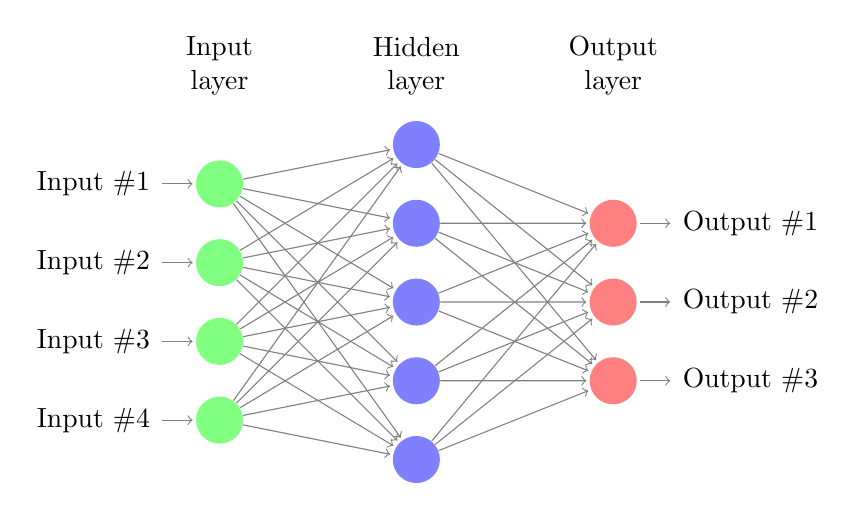
\begin{tikzpicture}[shorten >=1pt,->,draw=black!50, node distance=\layersep]
    \tikzstyle{every pin edge}=[<-,shorten <=1pt]
    \tikzstyle{neuron}=[circle,fill=black!25,minimum size=17pt,inner sep=0pt]
    \tikzstyle{input neuron}=[neuron, fill=green!50];
    \tikzstyle{output neuron}=[neuron, fill=red!50];
    \tikzstyle{hidden neuron}=[neuron, fill=blue!50];
    \tikzstyle{annot} = [text width=4em, text centered]

    % Draw the input layer nodes
    \foreach \name in {1,...,4}
        \node[input neuron, pin=left:Input \#\name] (I-\name) at (0,-\name) {};

    % Draw the hidden layer nodes
    \foreach \name in {1,...,5}
        \path[yshift=0.5cm]
            node[hidden neuron] (H-\name) at (\layersep,-\name cm) {};

    % Draw the input layer nodes
    \foreach \name in {1,...,3}
      \node[output neuron, pin={[pin edge={->}]right:Output \#\name}] (O-\name) at (2*\layersep,-0.5cm-\name cm) {};

    % Connect every node in the input layer with the hidden layer.
    \foreach \source in {1,...,4}
        \foreach \dest in {1,...,5}
            \path (I-\source) edge (H-\dest);

    % Connect every node in the hidden layer with the output layer
    \foreach \source in {1,...,5}
        \foreach \dest in {1,...,3}
            \path (H-\source) edge (O-\dest);

    % Annotate the layers
    \node[annot,above of=H-1, node distance=1cm] (hl) {Hidden layer};
    \node[annot,left of=hl] {Input layer};
    \node[annot,right of=hl] {Output layer};
\end{tikzpicture}
\caption[Beispielaufbau eines Neuronale Netzes]{Beispielaufbau eines Neuronale Netzes. Die Input Layer repräsentieren die Eingabe in das Netz. Hidden Layer sind versteckte Schichten im Modell. Die Ausgabe auf der linken Seite ist bei einer Klassifikation, Wahrscheinlichkeiten, bezogen auf die  zu erwartenden Label. Die Kanten zwischen den Schichten haben Gewichte anhand deren die Eingabe modifiziert wird (eigene Darstellung).}\label{cap:neuralnet}
\end{figure}\label{fig:neuralnet}

Das Training dieser Netze basiert auf Vorwärts- und Rückwärtsrechnen der Parameter an den Kanten und Knoten der Layer. Dabei läuft zuerst das Eingabebild alle Schichten des Neuronalen Netzes ab, welche Reihen von verschiedenen Transformationen ausführen. Das Ergebnis nach dem Durchlauf wird mit dem realen, zu erwartenden Ergebnis, verglichen. Diese ist innerhalb der Trainingsphase bekannt ist. Die Abweichung von diesem Vergleich, auch bekannt als Fehler (Loss), wird in der umgekehrten Richtung durch das Netzwerk geschickt. Die Gewichte an den Kanten zwischen den Layern werden anhand des Fehlers angepasst. So soll erreicht werden, dass das Netz sich im Verhalten der Ein- und Ausgabe konvergiert und der Loss abnimmt.

\section{Automatentheorie}\label{automatatheory}
Automaten sind wichtige Bestandteile der Informatik. In der Theoretischen Informatik ist die zu erfüllende Aufgabe so im folgenden definiert:

\begin{quote}
\glqq Die Aufgabe des Automaten besteht darin, eine Eingabe $w \in \{0, 1 \}\ast$ zu
durchlaufen (Buchstabe für Buchstabe), und die entsprechenden Transitionen
zwischen den Zuständen durchzuführen. Wenn die Eingabe komplett
durchlaufen wurde, also keine neuen Buchstaben mehr vorhanden sind, wird
das Eingabewort akzeptiert, sofern sich der Automat in einem akzeptierenden
Zustand befindet. Anderenfalls wird das Wort abgelehnt. Dies entspricht dem
weiter oben eingeführten Wortproblem. Man sagt, der Automat entscheidet
die Sprache.\grqq \cite{theororeticalinformatic}
\end{quote}

Die Eingabe $w$ muss sich nicht zwangsläufig auf den Wertebereich $\{0, 1 \}\ast$ beziehen. Aufgabengebiete solcher Maschinen beinhalten Steuerungsaufgaben, Mustererkennung in Daten, Netzwerkprotokolle, Sprachverarbeitung, Klassifizierungen und anderweitige Anwendungsmöglichkeiten. Es gibt zwei zu unterscheidende Hauptkategorien von Automatenklassen, die \acp{dea} und \acp{nea}.

Ein \ac{dea} ist formal komplett durch ein 5-Tupel $M = (Q, \Sigma, \delta, q_0, F)$ definiert. Das 5-Tupel für den \ac{dea} enthält folgende Komponenten:

\begin{itemize}
  \setlength\itemsep{-0.6em}
\item $Q$  ist eine endliche Zustandsmenge
\item $\Sigma$ ist ein endliches Alphabet
\item $\delta:Q \times \Sigma \rightarrow Q$ deterministische Übergangsfunktion
\item $q_0 \in Q$ ist der Startzustand
\item $F \subseteq Q$ Menge aller akzeptierten Endzustände
\end{itemize}


Ein \ac{nea} ist formal durch ein 5-Tupel $M = (Q, \Sigma, \delta, E, F)$ definiert. Der Unterschied zwischen \ac{dea} und \ac{nea} ist, dass beim \ac{nea} mehrere Startzustände vorhanden sein können und die Übergangsfunktionen nicht alle Formal definiert sein müssen. Ein \ac{nea} kann in einen \ac{dea} umgewandelt werden. Das 5-Tupel für den \ac{nea} enthält folgende Komponenten:

\begin{itemize}
  \setlength\itemsep{-0.6em}
\item $Q$  ist eine endliche Zustandsmenge
\item $\Sigma$ ist ein endliches Alphabet
\item $\delta:Q \times \Sigma \rightarrow P(Q)$ nicht-deterministische Übergangsfunktion
\item $E \subseteq Q$ die Menge der Startzustände
\item $F \subseteq Q$ Menge aller akzeptierten Endzustände
\end{itemize}



\clearpage
\section{Statistik}\label{statistics}
Um die verschiedenen Experimente statistisch vergleichen zu können, wird eine Wahrheitsmatrix bzw. Konfusionsmatrix $W$ (eng. Confusion Matrix) erstellt. Diese Matrix ist eine Auflistung aller Ergebnisse eines Trainingsschrittes (Epoch) der Neuronalen Netze. Dazu werden die vorhergesagten Klassen in die Zeile mit der realen Klasse in die Matrix eingetragen (siehe Abb. \ref{cap:conv_matrix}).

%The matrix in numbers
%Horizontal target class
%Vertical output class
\def\myConfMat{{
{110,  25,  30},  %row 1
{   0, 59,  31},  %row 2
{   5, 35,  90},  %row 3
}}

\def\classNames{{1, 2, 3}} %class names. Adapt at will

\def\numClasses{3} %number of classes. Could be automatic, but you can change it for tests.

\def\myScale{1.5} % 1.5 is a good scale. Values under 1 may need smaller fonts!

\begin{figure}[!b]
\begin{center}
\begin{tikzpicture}[scale = \myScale,%font={\scriptsize}, %for smaller scales, even \tiny may be useful
  ]
\tikzset{vertical label/.style={rotate=90,anchor=east}}   % usable styles for below
\tikzset{diagonal label/.style={rotate=45,anchor=north east}}

\foreach \y in {1,...,\numClasses} %loop vertical starting on top
{
    % Add class name on the left
    \node [anchor=east] at (0.4,-\y) {\pgfmathparse{\classNames[\y-1]}\pgfmathresult};
    \foreach \x in {1,...,\numClasses}  %loop horizontal starting on left
    {
%---- Start of automatic calculation of totSamples for the column ------------
    \def\totSamples{0}
    \foreach \ll in {1,...,\numClasses}
    {
        \pgfmathparse{\myConfMat[\ll-1][\x-1]}   %fetch next element
        \xdef\totSamples{\totSamples+\pgfmathresult} %accumulate it with previous sum
        %must use \xdef fro global effect otherwise lost in foreach loop!
    }
    \pgfmathparse{\totSamples} \xdef\totSamples{\pgfmathresult}  % put the final sum in variable
%---- End of automatic calculation of totSamples ----------------

    \begin{scope}[shift={(\x,-\y)}]
        \def\mVal{\myConfMat[\y-1][\x-1]} % The value at index y,x (-1 because of zero indexing)
        \pgfmathtruncatemacro{\r}{\mVal}   %
        \pgfmathtruncatemacro{\p}{round(\r/\totSamples*100)}
        \coordinate (C) at (0,0);
        \ifthenelse{\p<50}{\def\txtcol{black}}{\def\txtcol{white}} %decide text color for contrast
        \node[
            draw,                 %draw lines
            text=\txtcol,         %text color (automatic for better contrast)
            align=center,         %align text inside cells (also for wrapping)
            fill=black!\p,        %intensity of fill (can change base color)
            minimum size=\myScale*10mm,    %cell size to fit the scale and integer dimensions (in cm)
            inner sep=0,          %remove all inner gaps to save space in small scales
            ] (C) {\r};     %text to put in cell (adapt at will)
        %Now if last vertical class add its label at the bottom
        \ifthenelse{\y=\numClasses}{
        \node [] at ($(C)-(0,0.75)$) % can use vertical or diagonal label as option
        {\pgfmathparse{\classNames[\x-1]}\pgfmathresult};}{}
    \end{scope}
    }
}
%Now add x and y labels on suitable coordinates
\coordinate (yaxis) at (-0.3,0.5-\numClasses/2);  %must adapt if class labels are wider!
\coordinate (xaxis) at (0.5+\numClasses/2, -\numClasses-1.25); %id. for non horizontal labels!
\node [vertical label] at (yaxis) {Reale Klasse ($r$)};
\node []               at (xaxis) {Prediction aus den Neuronalen Netz ($p$)};
\end{tikzpicture}
\caption[Beispiel einer Warheitsmatrix $W$]{Beispiel einer Wahrheitsmatrix. Das Ergebnis aus den Neuronalen Netzen wird einzeln mit den richtigen Ausgabewert verglichen und in die Zeile mit +1 eingetragen (eigene Darstellung).}\label{cap:conv_matrix}
\end{center}
\end{figure}\label{fig:conv_matrix}

Durch die Matrix, sind fünf Metriken bestimmbar. Sensitivität, welches die Wahrscheinlichkeit angibt, anhand deren ein Objekt richtig klassifiziert wurde. Das Gegenteil ist die Spezifität. Diese gibt an, mit welcher Wahrscheinlichkeit ein Objekt falsch klassifiziert wird. Als weitere Werte lassen sich Spezifität und Segreganz (Positiver und negativer Vorhersagewert) berechnen. Diese geben den Anteil der korrekt klassifizierten an der Gesamtheit der klassifizierten Ergebnisse positiv und negativ an. Der F1-Wert ist dabei das harmonische Mittel zwischen Sensitivität und Genauigkeit.

Um für die statistischen Merkmale Sensitivität, Genauigkeit, Spezifität, Segreganz und F1 für die Matrix als Mittelwert berechnen zu können, ist für alle Klassen zuerst notwendig, die Einzelwerte für diese zu berechnen. Danach werden alle Klassen zusammenaddiert und der Mittelwert über ihnen gebildet. Die spezifischen Werte für eine Klasse $g$, die Wahrheitsmatrix $W$, die Reihe $r$ und Spalte $p$ können nach den Formeln (\ref{eg:tpr} - \ref{eg:f1}) ausgerechnet werden \cite{matrix_calc_paper}:


\begin{alignat}{1}
  Sensitivität (TPR) &= \frac{TP}{TP + FN} = \frac{W_{g, g}}{\sum_{n=1}^{n} r_{g}}                \label{eg:tpr}\\
  Genauigkeit (PPV)  &= \frac{TP}{TP + FP} = \frac{W_{g, g}}{\sum_{n=1}^{n} p_{g}}                \label{eg:ppv}\\
  Spezifität (TNR)   &= \frac{TN}{TN + FP} = \frac{W_{\neg g, \neg g}}{\sum_{n=1}^{n} r_{\neg g}} \label{eg:tnr}\\
  Segreganz (NPV)    &= \frac{TN}{TN + FP} = \frac{W_{\neg g, \neg g}}{\sum_{n=1}^{n} p_{\neg g}} \label{eg:npr}\\
  F1                 &= \frac{2 * PPV * TPR}{PPV + TPR}                                           \label{eg:f1}
\end{alignat}


Die Diagonalpositionen der oben gezeigten Matrix repräsentieren alle Richtig-Positiv Klassifizierungen der respektiven Klasse. Anhand dieser Metriken kann so herausgefunden werden, ob ein Neuronales Netz in eine Über- bzw. Unteranpassung (eng. Over- und Underfitting) hineinläuft. Auch ein Indiz für einen guten Lernvorschritt ist, wenn der F1-Wert quasi asymptotisch Richtung 1 annähert. In der Szene des Maschinellen Lernens ist der F1-Wert der Maßstab.


























\chapter{Stand der Technik}\label{std}
Im folgenden Kapitel soll der momentane  Stand der Technik für die zugrunde liegende Aufgabenstellung erläutert werden. Dabei werden 2 verschiedene Vorangehensweisen kurz erläutert. Der Abschnitt \ref{segmentation} veranschaulicht dabei die Graduierung der Fazialisparese durch die Anwendung von Segmentierung zur Extraktion der wichtigsten Gesichtseigenschaften. Eine andere Herangehensweise ist mit Videoframes vergleichsbasiert mit einer aufgenommenen Referenzstellung und anderen Posen den \ac{hb_grade} festzustellen (Kapitel \ref{compare}).

\section{Segmentierung basierte Methode}\label{segmentation}
Eine Methode zur Erkennung einer Fazialisparese ist die Anwendung von Segmentierung, um die Gesichtsmerkmale aus den Bildern zu extrahieren. Diese semantischen Merkmale enthalten räumliche Eigenschaften des/der Patient*in, die für die Klassifikation des Schweregrades, aus optischer Sicht, unerlässlich sind.

\begin{figure}[!b]
\centering
\resizebox{0.95\textwidth}{!}{%
\begin{tikzpicture}[->,>=stealth',shorten >=1pt,auto,node distance=2.5cm,semithick,scale=0.50]
  \tikzstyle{every state}=[fill=cyan,draw=black,text=black]

  \definecolor{in_out_col}{RGB}{60,199,215}
  \tikzstyle{level0} = [rectangle, draw, fill=in_out_col, text width=8cm, text centered, rounded corners, minimum height=1cm, minimum width=8cm]

  \definecolor{enc_col}{RGB}{199,215,60}
  \tikzstyle{level1} = [rectangle, draw, fill=enc_col, text width=4cm, text centered, inner sep=1pt  , minimum height=2cm, minimum width=2cm]

  \tikzstyle{level2} = [rectangle, draw, fill=blue!20, text width=5cm, text centered, rounded corners, minimum height=1cm, minimum width=5cm]

  \tikzstyle{level3} = [rectangle, draw, fill=green!40!blue!20, text width=4cm, text centered, inner sep=1pt  , minimum height=3cm, minimum width=3cm]

  \definecolor{att_mod_col}{RGB}{60, 142, 215}
  \tikzstyle{level3_att_mod} = [rectangle, draw, fill=att_mod_col, text width=3cm, text centered, inner sep=1pt  , minimum height=0.5cm, minimum width=2.5cm]

  \definecolor{enc_2_col}{RGB}{215,60, 199}
  \tikzstyle{level3_2} = [rectangle, draw, fill=enc_2_col, text width=4cm, text centered, inner sep=1pt  , minimum height=3cm, minimum width=3cm]

  \tikzstyle{level4} = [rectangle, draw, fill=blue!20, text width=3cm, text centered, rounded corners, minimum height=1.5cm, minimum width=3cm]

  \tikzstyle{level5} = [rectangle, draw, fill=in_out_col, text width=4cm, text centered, rounded corners, minimum height=1.5cm, minimum width=4cm]



  \node[level0]    (Z0)[rotate=90]                                 {\textbf{Eingabe}};
  \node[level1]    (A) [right of=Z0, xshift=1.5cm]                 {\textbf{Encoder E1} \\ vollständiges \\ Faltungsnetzwerk};
  \node[level2]    (B) [right of=A      , xshift=1.5cm, rotate=90] {Featuremap};
  \node[level3]    (C) [above right of=B, xshift=2cm , yshift=1cm, text depth=2cm] {Attention Modul};
  \node[level3_att_mod]    (C1) [above right of=B, xshift=2cm , yshift=1.3cm] {};
  \node[level3_att_mod]    (C2) [above right of=B, xshift=2cm , yshift=0.7cm] {};
  \node[level3_att_mod]    (C3) [above right of=B, xshift=2cm , yshift=0.1cm] {};

  \node[level4]    (D) [right of=C      , xshift=1.5cm, rotate=90] {Pixel für Pixel \\ Klassifikation};
  \node[level3_2]  (E) [below right of=B, xshift=2cm, yshift=-1cm] {\textbf{Encoder E2} \\ Faltungsnetzwerk als Dimensionskompressor};
  \node[level4]    (F) [right of=E      , xshift=1.5cm, rotate=90] {Grad \\ Klassifizierer};

  \node[level5]    (Z1)[right of=D      , xshift=1.5cm, rotate=90] {\textbf{Ausgabe} \\ \textbf{Segmentierung}};
  \node[level5]    (Z2)[right of=F      , xshift=1.5cm, rotate=90] {\textbf{Ausgabe} \\ \textbf{Klassifizierung} \\ $[I, II, III, IV, V, VI]$};


  \path (A)  edge [line width=0.8mm,  green!70, bend left= 15] node {} (B)
        (A)  edge [line width=0.8mm,   blue!70, bend left=-15] node {} (B)
        (B)  edge [line width=0.8mm,    red!70               ] node {} (A)

        (B)  edge [line width=0.8mm,  green!70, bend left=15]  node {} (C)
        (C)  edge [line width=0.8mm,    red!70, bend left=15]  node {} (B)
        (C)  edge [line width=0.8mm,  green!70, bend left=15]  node {} (D)
        (D)  edge [line width=0.8mm,    red!70, bend left=15]  node {} (C)
        (D)  edge [line width=0.8mm,  green!70, bend left=15]  node {} (Z1)
        (Z1) edge [line width=0.8mm,    red!70, bend left=15]  node {} (D)


        (B)  edge [line width=0.8mm,   blue!70              ] node {} (E)
        (E)  edge [line width=0.8mm,   blue!70, bend left=15] node {} (F)
        (F)  edge [line width=0.8mm, bend left=15           ] node {} (E)
        (F)  edge [line width=0.8mm,   blue!70, bend left=15] node {} (Z2)
        (Z2) edge [line width=0.8mm, bend left=15           ] node {} (F)

        (Z0) edge [line width=0.8mm,  blue!70, bend right=30] node {}(E)
        (Z0) edge [line width=0.8mm,  blue!70, bend left=-15] node {} (A)
        (Z0) edge [line width=0.8mm,  green!70, bend left=15] node {} (A);
\end{tikzpicture}
}%
\caption[Darstellung der Flowchart vom Paper Automatic Facial Paralysis Evaluation Augmented by a Cascaded Encoder Network Structure.]{Darstellung der Flowchart vom Paper Automatic Facial Paralysis Evaluation Augmented by a Cascaded Encoder Network Structure. Die blauen und grünen Pfeile ist der Evaluierungsdatenfluss. Rot und Schwarz jeweils der Trainingsfluss \cite{detection_fp2}.}\label{cap:paper_1}
\end{figure}\label{fig:paper_1}

Der Experimentaufbau von T. Wang et al. enthaltet ein kaskadierenden Encoder Netzstruktur zur Ausführung der Bewertung der Fazialisparese (siehe Abb. \ref{cap:paper_1}). Auf Basis von Neuronalen Netzen, besteht dieser Aufbau aus zwei Komponenten. Semantischen Segmentierung von Gesichtsattributen und ein Klassifikationsnetz über eine vorher extrahierte Funktionskarte (Encoder). Dieser Encoder komprimiert die Bilddaten Pixel für Pixel durch ein Faltungsnetzwerk (eng. Convolution). Verwendet wird dazu ein vortrainiertes ResNet-101 ohne Verkleinerung des Eingabemateriales. Als Training für den Encoder diente in der Studie ein Mix aus mit und ohne Fazialsparese, um ihn separat vom Rest vorab zu trainieren. Dadurch konnte genug räumliche Informationen über die Gesichter gewonnen werden, die für die Segmentierung und die Graduierung benötigt werden. Die daraus enthaltenen Daten aus dem Encoder dienen als Feature für die Segmentierung und die direkte Klassifikation des Grades nach House-Brackmann. Segmentierung ist eine Pixel für Pixel Klassifikation über das gesamte Bild. Die Gesichtspartien können so für die betrachteten Teilregionen der House-Brackmann Skala eingefärbt werden. Als Ausgabe dient die Klassifizierung und das segmentierte Bild, der für die weitere klinische Einschätzung durch einen Facharzt*in zurückgeliefert werden. Durch die Anwendung des kaskadierenden Trainings ist so ein F1 Wert von 95.85\% erzielt \cite{detection_fp2}.

Der große Vorteil von dieser Methode ist, dass die Segmentierung getrennt von der Graduierung eine Rückgabe liefert. Aus der Segmentierung der Bilder kann so erkannt werden, welche Bereiche des Bildes für die Dedektion genutzt wurde und ob diese überhaupt die richtigen Regionen der Gesichtsparien sind. Auch können Rückschlüsse auf die enthaltene Featuremap geschlossen werden, die für den Klassifizerier des Grades auch von Relevanz ist, da Segmentierung und Klassifizierung die selbe Featuremap benutzen.



\section{Vergleichsbasierte Erkennung anhand eines Videos}\label{compare}
\begin{figure}[!t]\centering
\begin{tikzpicture}[->,>=stealth',shorten >=1pt,auto,node distance=2.5cm,semithick]
  \tikzstyle{every state}=[fill=cyan,draw=black,text=black]

  \tikzstyle{level1} = [rectangle, draw, fill=green!40!blue!20, text width=12cm, text centered, inner sep=1pt  , minimum height=1.3cm]
  \tikzstyle{level2} = [rectangle, draw, fill=blue!20, text width=4cm, text centered, rounded corners, minimum height=2.5cm, minimum width=4cm]
  \tikzstyle{level3} = [rectangle, draw, fill=green!40!blue!20, text width=8cm, text centered, inner sep=1pt  , minimum height=1.3cm]
  \tikzstyle{level4} = [rectangle, draw=white, fill=white, text width=1cm, text centered, minimum height=0.1cm, minimum width=0.1cm]

  \node[level1]         (A)        {Input Video};
  \node[level2]         (B) [below left  of=A, yshift=-2cm, rotate=90] {Beleuchtungs- \\ kompensationsfaktor \\ $lum$};
  \node[level2]         (C) [below right of=A, yshift=-2cm, rotate=90] {relative Vertikale \\ Verschiebung zwischen\\ Referenz und Peak \\ $Sym_y$};
  \node[level2]         (D) [left  of=B, xshift=-1cm, rotate=90]       {$\frac{argmin(mag_{right}, mag_{left})}{argmax(mag_{right}, mag_{left})}$ \\ mit $mag_{right}, mag_{left}$ als relative Pixelveränderung zwischen \\ Referenz und Peak};
  \node[level2]         (E) [right of=C, xshift=1cm, rotate=90]        {relative Stärke \\ des Unterschiedes zwischen \\ Referenz und Peak \\ $Sym_r$};
  \node[level3]         (F) [below right of=B, yshift=-2cm] {k-Nearest-Neighbour (k-NN) \\ Neuronales Netz (NN) \\ Support Vector Machine (SVM)};

  \node[level4]         (Z2) [right of=F, xshift=3cm]        {};

  \path (A) edge [bend right=15] node {} (B)
            edge [bend left=15] node {} (C)
            edge [bend right=15] node {} (D)
            edge [bend left=15] node {} (E)
        (B) edge [bend right=15] node {} (F)
        (C) edge [bend left=15] node {} (F)
        (D) edge [bend right=15] node {} (F)
        (E) edge [bend left=15] node {} (F)

        (F) edge [out=0   , in=180] node [right, xshift=0.3cm, align=left]                {Output \\ H-B Grad $[I, ..., VI]$} (Z2);

\end{tikzpicture}
\caption[Nachgestellte Interpretation der beschriebenen Vorgehensweise für]{Nachgestellte Interpretation der beschriebenen Vorgehensweise. Eingabefaktoren für die im Paper verwendeten sind Pixeldichte, Beleuchtungsfaktor, relative Vertikale und Stärke jeweils auf ein Referenzframe und dem Peak im Video betrachtet \cite{detection_fp1}.}\label{cap:paper_2}
\end{figure}\label{fig:paper_2}


Eine weitere Möglichkeit neben der Segmentierung ist es, aus einem Video herausgeschnittene Frames mit einer Referenz zu vergleichen. Dazu werden fünf unterschiedlichste Gesichstsbewegungen durchgeführt. Diese sind Augenbraun heben, Augen sanft sowie forciert schließen, Nase rümpfen und lächeln. Die Viedeosequenz beginnt mit der Referenzansicht, wobei sich der/die Patient*in in Ruheposition befindet. Nach jeder Bewegung kehren er/sie auch wieder in die Ausgangsposition zurück. Anhand von Framesubstraktion können so dann die einzelnen Positionen aus dem Video entnommen werden.

Nachdem die einzelnen Posen aus dem Video herausgezogen worden sind, werden die einzelnen Gesichtsregionen lokalisiert. Um die Gesichtskonturen zu detektieren wird ein Sobel-Filter angewendet. Dieser nutzt eine Faltungsoperation, die aus dem Bild einen Gradienten erzeugt. Die Bereiche mit der größten Intensität, also den Stellen wo sich die Helligkeit am stärksten ändert, werden hervorgehoben. Die anderen Bereiche werden mit Grauwerten dargestellt. Alle entscheidenden Features des Gesichtes (Augenbraun, Nase, Mund und Augen) sind dunkler als die normale Hautfarbe. Durch Eine Verschiebung der Pixelwerte lassen sich diese hervorheben und deren absolute Position im Bild feststellen.

Anhand dessen werden vier Eingabewerte berechnet, die für eine Klassifikation mit einem Neuronalen Netz benötigt werden (siehe Abb. \ref{cap:paper_2}). Dazu zählen die relative Pixelveränderung in den einzelnen Regionen, die sich von der Ruheposition bis zu dem Höhepunkt der dargestellten Bewegung ausgerechnen lässt. Auch der Beleuchtungskompensationsfaktor spielt eine Rolle. Dieser misst die Unterschiede zwischen der dysfunktionalen und der normalen Seite, um die Intensität und Ausprägung der Funktionsstörung ermitteltn zu können. Die weiteren beiden Eingabewerte sind Faktoren, die sich aus dem optischen Fluss der Regionen darstellen lässt. Dazu werden Vektoren genutzt, die von der Spiegelachse - dem Nasenrücken - und beiden Gesichtshälften in einem Raster die Richtungsänderungen und Falten im Gesicht zeigen sollen. Aus dieser Grafik werden einmal die Symmetrie in vertikaler Richtung und die Stärke dieser Vektoren berechnet. Diese genannten Faktoren dienen als Eingabe in ein Klassifikationsnetzwerk, dass nach der House-Brackmann Skala den Grad der Parese feststellt \cite{detection_fp1}.
